\chapter{机器学习与深度学习简介}\label{chapter_machinelearning}
\graphicspath{{chapter2/figure/}}
\bibliographystyle{unsrt}

本章笔者将对机器学习领域的一些基本思想做一个介绍,尤其是介绍与本文算法相关的背景知识。在机器学习的基础上,笔者将对目前深度学习的一些主流方向做一个简介。

\section{机器学习}

\subsection{机器学习简介}

\subsubsection{定义与引例}

机器学习被定义为一门“让计算机在没有被准确、具体地编程的情况下获得学习能力”的学科。
机器学习鉴于一种朴素的思想:\uline{通过机器自动分析数据中的规律,并作出相应的预测}。 

一个最简单的“学习”案例便是曲线的的“拟合”过程。笔者想通过一个“拟合”实例来说明机器学习的基本思想。

假设我们有两个实值变量x、t,其满足关系
\begin{equation}
\label{eqn:random}
y = \sin(2\pi x) + \epsilon
\end{equation}

其中$\epsilon$是一个服从Gaussian分布的随机值。

假设我们有m组(x,y)的观测值$x \equiv (x_1, x_2, ..., x_m)^T, y \equiv (y_1, y_2, ..., y_m)^T$,图\ref{fig:fitting}为m=10时的数据点和原Sine函数。

\begin{figure}[htbp]
   \centering
   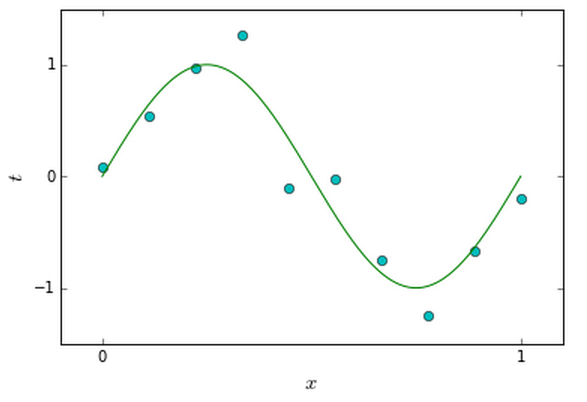
\includegraphics[width=0.5\textwidth]{SineFitting.png} % requires the graphicx package
   \caption{拟合的原数据点,真实的Sine函数}
   \label{fig:fitting}
\end{figure}

图\ref{fig:polyfitting}通过三阶多项式函数进行拟合的结果。通过已知的10个数据点,我们获得了一条多项式曲线,通过这条曲线便可以推断、预测已知数据点之外的点的信息。

\begin{figure}[htbp]
   \centering
   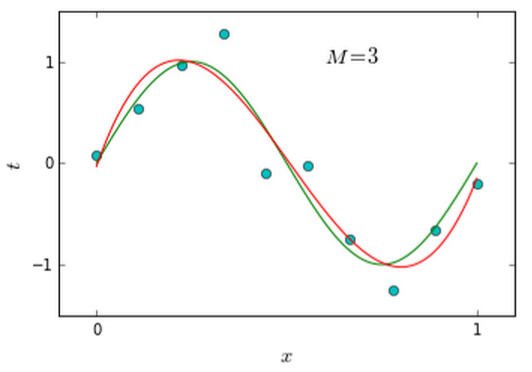
\includegraphics[width=0.5\textwidth]{PolyFitting.png} % requires the graphicx package
   \caption{多项式“拟合”:对真实情况进行预测、推断}
   \label{fig:polyfitting}
\end{figure}

在本例中,机器的学习过程便转化为了\uline{如何产生合适的拟合曲线的问题}。我们假设多项式满足以下形式:
\begin{equation}
h(x,\mathbf{w}) = w_0 + w_1x + w_2x^2 + ... + w_Mx^M = \sum_{j=0}^M w_j x^j
\end{equation}

其中$h(x,\mathbf{w})$为假设预测值,M为多项式阶数,$\mathbf{w} = (w_0, w_1, ..., w_M)$ 表示多项式的系数。

首先,我们就要对曲线“\textbf{合适}”的概念做一个分析。什么是合适的曲线?一个自然的观点便是,曲线应当能够\uline{较好地符合已有的数据}。为了衡量曲线符合已有数据的程度,我们根据曲线预测值和真实值的偏差的函数进行描述。一种常见的偏差的度量是采用\uline{偏差的平方值}(取平方值加和是严格基于数据独立同分布,围绕真实值正态分布的极大似然概率推导得出的\cite{standford_machine_learning_cs229})。于是,我们定义\textbf{损失函数}如下:

\begin{equation}
E(\mathbf{w}) = \dfrac{1}{2} \sum^m_{i=1} (h(x, \mathbf{w}) - y_i )^2
\end{equation}

其中$\frac{1}{2}$是为了之后计算的方便而加上的。

我们的目标便从拟合曲线转变为了\uline{选择合适的$\mathbf{w}$,使得损失函数$E(\mathbf{w})$最小}。

常见的一种方法是,分析此损失函数$E(\mathbf{w})$的梯度,发现其为$\mathbf{w}$的线性函数,即存在唯一极小值点,此即我们寻找的最优点:

\begin{equation}
\dfrac{\partial E(\mathbf{w})}{w_j} = \sum^m_{i=1} ( \sum^m_{j=0} w_j x^j_i - y_i ) x^j_i = 0
\end{equation}

上式即“最小二乘法”的基本原理公式。

然而,在大多数时候,我们的损失函数不具有以上良好的结构:具有多个极小值点;微分性质不佳;甚至没有明确的函数定义。 

于是我们产生了一种基于“学习”的思想:

\uline{先寻找一个或者多个试探点$\{w_j\}$; 再衡量其损失函数的表现; 最后根据原来试探点的表现更新试探点的位置}。 

进行以上迭代,直到得到一个满足要求的点为止。

在以上“学习”过程中,有几个不可或缺的要素:
\begin{itemize}
\item 学习的任务T(Task):在以上实例中,任务的确认即为\uline{描述什么是“合适”的曲线}:函数预测值和原训练点的满足程度;
\item 结果的观测P(Performance):以上实例中,即为\uline{损失函数$E(\mathbf{w})$的具体形式的确定};
\item 学习的经验E(Experience):实例中体现为:\uline{拟合函数形式的假设}(多项式函数)以及\uline{更新规则的制定}。
\end{itemize}

一个被广泛引用的机器学习的定义是\cite{mitchell1997machine}:假设存在一个任务T,已有的经验E,和对于结果的观测P;如果一个机器通过经验E改善了其在任务T中的表现(通过P来观测),我们就说机器进行了学习。


%最早的机器学习研究源于统计学里面的一些方法:回归分析、主元分析、聚类问题、Bayesian推断等等。 

相比较于普通的静态算法(比如最小二乘法)而言,机器学习更加看重“数据驱动”(data-driven),根据数据变化不断调整自己的推断、预测。


\subsubsection{机器学习的分类}
机器学习按照学习形式主要划分为\uline{监督学习、非监督学习}两大类。其主要的区别就在于学习的任务T(Task)的区别:

\begin{itemize}
\item 监督学习中,训练数据集含有训练的标签值(比如说实例中的y值);学习的任务一般为\uline{提高函数预测值$h_i$和原训练点标签值$y_i$的满足程度};
\item 非监督学习中,训练数据集不带有标签;学习的任务可能为:寻找数据的聚类;主元分析等等。(后面会展开讲)
\end{itemize}

除了以上的两类机器学习,还存在着\uline{半监督学习、强化学习}的学习类型。

半监督学习指的是数据集中存在一部分数据具有训练标签(往往更加贴近于实际情况),而大部分数据是没有标签的情况下进行数据分析预测; 

强化学习是目前的一个新兴领域,其主要思想是结果的观测P不再基于具体的损失函数$E(\mathbf{w})$,而是基于一个刺激信号(比如下围棋时获得胜利能够赢得奖励)。

本章主要围绕较为成熟的监督学习、非监督学习理论展开介绍。

\subsection{监督学习}
根据上一节,我们已知,监督学习为提高函数预测值$h_i$和原训练点标签值$y_i$的满足程度
 根据数据集的具体形式,监督学习可以具体表现为:
\begin{enumerate}
\item 回归问题: 数据集的自变量X、因变量y(标签)\textbf{均连续};
\item 分类问题: 数据集的自变量X\textbf{连续},因变量y(标签)\textbf{离散};
\item 序列标记问题: 数据集自变量X、因变量y(标签)\textbf{均离散};
\end{enumerate}
以下我们主要讨论回归问题与分类问题。 

我们先分析常规回归问题的处理方法,再讨论利用Sigmoid函数实现分类问题的处理;当自变量X维数增加时,应用常规的高维优化方法将变得非常困难,我们将讨论基于此发展的神经网络算法,这将是后来深度学习算法的重要基础;最后我们将简要地介绍机器学习的基本数学基础:Bayes理论。

\subsubsection{优化方法之梯度下降法}
我们将回归问题进一步抽象:为了不失普遍性,我们设自变量有两个,因变量有一个;数据空间为($y: x_1, x_2$)。训练集为m组数据($y_i: x_{1i}, x_{2i} (i=1\sim m)$)。 

那么任何一个回归问题都可以分为三个部分:

\begin{enumerate}
\item 数据结构的先验假设: y与x的函数关系假设; 最终将会被抽象为一个线性表达式

\begin{equation}
\begin{aligned}
h(x,\mathbf{w}) = & w_0 + w_{10} x_1 + w_{20} x_1^2 + ... + w_{M0} x_1^M + w_{01} x_2 + w_{02} x_2^2 + ... \\
& + w_{0N} x_2^M + w_{11} x_1 x_2 + ...+ w_{ij} x_1î x_2^j + ... + w_{k} f(x_1, x_2)
\end{aligned}
\end{equation}

其中y表示为$x_1$, $x_2$的幂指数项,$x_1, x_2$的交叉幂项,以及某些先验的$f(x_1, x_2)$非幂项(比如$\sqrt{x_1}$)。

\item 损失函数$E(\mathbf{w})$形式的确认: 对于回归问题,我们采用训练集真实数据$y_i$同模型预测值$h_i$的差值的平方和作为损失函数。 更加严格地,为了防止“过拟合”现象的发生,我们在损失函数后附上正则化项
\begin{equation}
\label{eqn:costfunction}
E(\mathbf{w}) = \dfrac{1}{2} \sum^N_{i=1} (y_i(x, \mathbf{w}) - t_i )^2 + \dfrac{\lambda}{2} ||w||^2
\end{equation}

\item 损失函数极小化采用的优化方法。 比如前面提到的利用一阶导数为0寻找极小值点的最小二乘法。
\end{enumerate}

本小节我们讨论另外一种常见的优化方法:\textbf{梯度下降法}。梯度下降法代表了含导数优化方法的典型思想,在机器学习优化中被广泛应用。

梯度下降的基本思想是:不断地更新$\mathbf{w}$使$E(\mathbf{w})$变小;利用导数去判别更新$\mathbf{w}$的方向和长度,逼近极值点的位置。具体的更新规则为:

\begin{equation}
w_j := w_j -\alpha \dfrac{\partial}{\partial w_j} E(\mathbf{w})
\end{equation}

其中$\alpha$称为\uline{学习速率},是一个人为的参数。

在一个梯度下降进行学习的过程中,我们基于当前的$\mathbf{w}$进行预测值h的计算,并且计算其损失函数$E(\mathbf{w})$;再由损失函数及其梯度更新$\mathbf{w}$;循环以上步骤,直到满足停止条件(比如w基本不变)为止。


对于公式\ref{eqn:costfunction}形式的损失函数,其导数值为:
\begin{equation}
\dfrac{\partial}{\partial w_j} E(\mathbf{w}) = \dfrac{\partial}{\partial w_j} (\dfrac{1}{2} \sum^m_{i=1} (h_i(x, \mathbf{w}) - y_i )^2 + \dfrac{\lambda}{2} w_j^2 =\\
 \sum^m_{i=1} (h_i(x, \mathbf{w}) - y_i ) \dfrac{\partial}{\partial w_j} h_i(x, \mathbf{w}) + \lambda w_j
\end{equation}

我们通过以上梯度下降法和较为普适的线性模型,就可以较为方便地进行低维度回归问题的学习了。更严格的回归问题讨论详见\cite{standford_machine_learning_cs229}。

在基于一阶导数的优化方法中,有很多基于梯度下降法而发展出的方法。如“共轭梯度法”、“BFGS”法,“L-BFGS”法,他们往往比梯度下降法更快,并且不容易进入局部极小值点。在此不赘述。\cite{wikipedia_BGFS_algorithm}

\subsubsection{Sigmoid分类实现方法}
本节我们讨论分类问题的处理方法。 我们首先讨论二分类问题,即数据标签${t_i}$只有两种取值的情况。不失普遍性,我们假设${t_i}$取值为0或者1。

我们仍然可以套用之前回归模型的处理方法:仍然假设$E(\mathbf{w}) = \dfrac{1}{2} \sum^m_{i=1} (h_i(x, \mathbf{w}) - y_i )^2 + \dfrac{\lambda}{2} ||w||^2$,其中$y_i$的值取0或者1;通过$h_i(x,\mathbf(w))$表达式的值来确定h的大小。 然而,实验证明这样的效果并不理想,h的值不能总是很好地收敛于0,1旁边,训练处的模型y值较为分散。

一种朴素的改进方案是,不再通过连续值$h_i$来表示预测值,而是对其进行\textbf{后处理},将其处理成\uline{间断值}。比如说,设置一个变量$d_i$,其定义为:
\begin{equation}
d_i(h_i(x,\mathbf{w})) == \left\{
\begin{aligned}
 & 1  & h_i > 0.5 \\
 & 0  & h_i < 0.5 \\
\end{aligned}
\right.
\end{equation}

此模型称为“感知机”模型。\cite{wikipedia_perceptron}历史上“感知机”模型曾经是分类的主流方法。 

然而,此方法的缺点非常明显:\uline{$d_i(h_i)$不是一个微分性质良好的函数,不能够进行梯度下降法的优化计算}。

基于此,我们想到了用一个接近于“感知机”,但具有良好微分性质的函数来后处理$h_i$,这样便能得到较好的分类结果。

一个常见的“分类”函数称为Sigmoid函数,其表达式为:
\begin{equation}
d_i(h_i) = \dfrac{1}{1+e^{-d_i}}
\end{equation}

为了统一符号,我们在此改变符号记法,用$h$表示最终的预测值(即处理后的d值),而用$z$表示后处理之前的线性加和值(原h值),即:
$$ h(x,\mathbf{w}) = h(z(x,\mathbf{w})) = g(z) = \dfrac{1}{1 + e^{-z}}$$

其形状如图所示:

\begin{figure}[htbp]
   \centering
   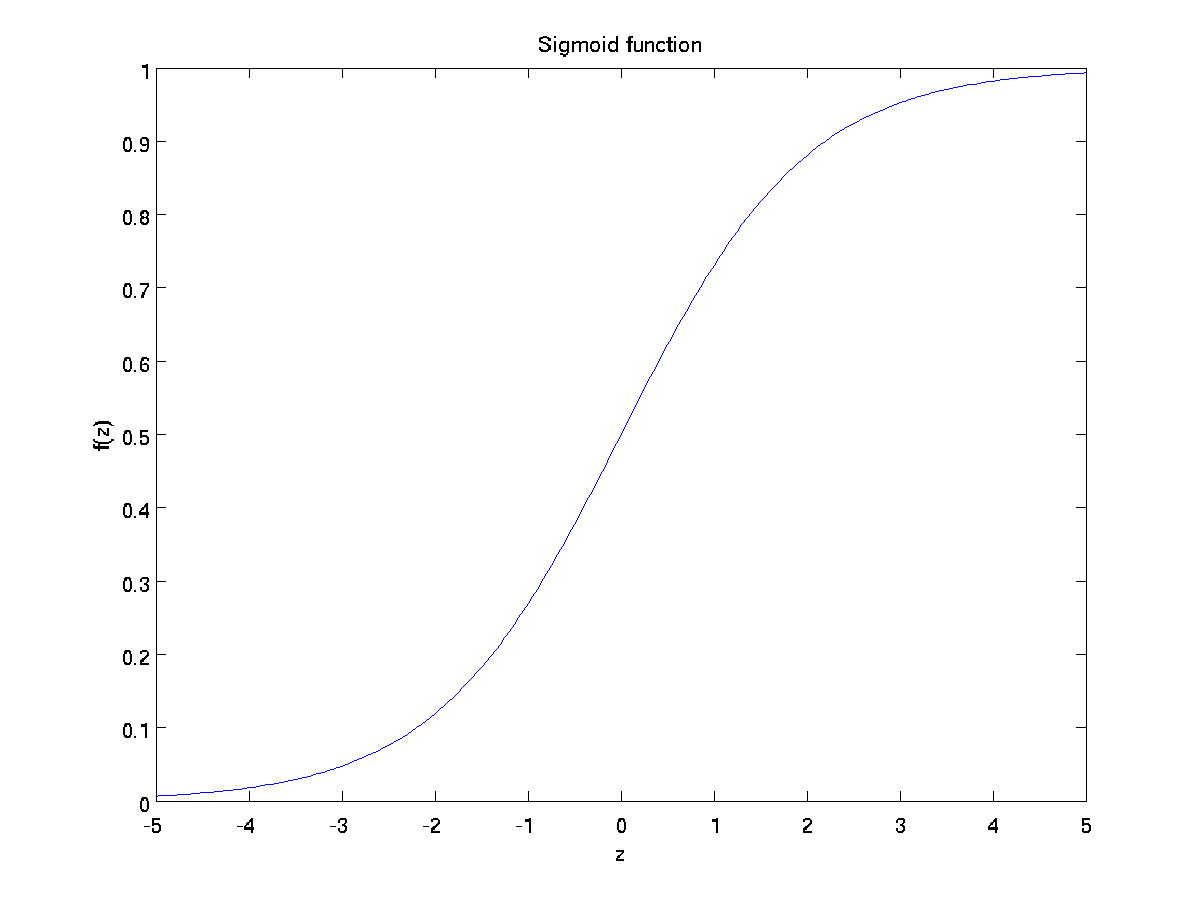
\includegraphics[width=0.6\textwidth]{SigmoidFunction.png} % requires the graphicx package
   \caption{Sigmoid函数的形状}
   \label{fig:sigmoid}
\end{figure}

我们称,$h$的值表示其归为分类‘1’的可信度。相反,其归为‘0’的可信度表示为$1 - h$。可见,当$z$大于0时,$h$的值大于0.5;反之$h$的值小于0.5。

那么,在训练的过程中,我们用$h$替代$z$作为优化的因变量,损失函数写为:(仍然通过极大似然法求得,考虑先取对数\cite{standford_machine_learning_cs229})

\begin{equation}
\begin{aligned}
& E(\mathbf{w}) = \dfrac{1}{m} \sum^m_{i=1} Cost(h(x^{(i)}),y^{(i)}) \\
& Cost(h(x^{(i)}),y^{(i)}) = \left\{
\begin{aligned}
 & -log(h(x))   & y = 1 \\
 & -log(1-h(x)) & y = 0 \\
\end{aligned}
\right.
\end{aligned}
\end{equation}

损失函数的图像如下:
\begin{figure}[htbp]
   \centering
   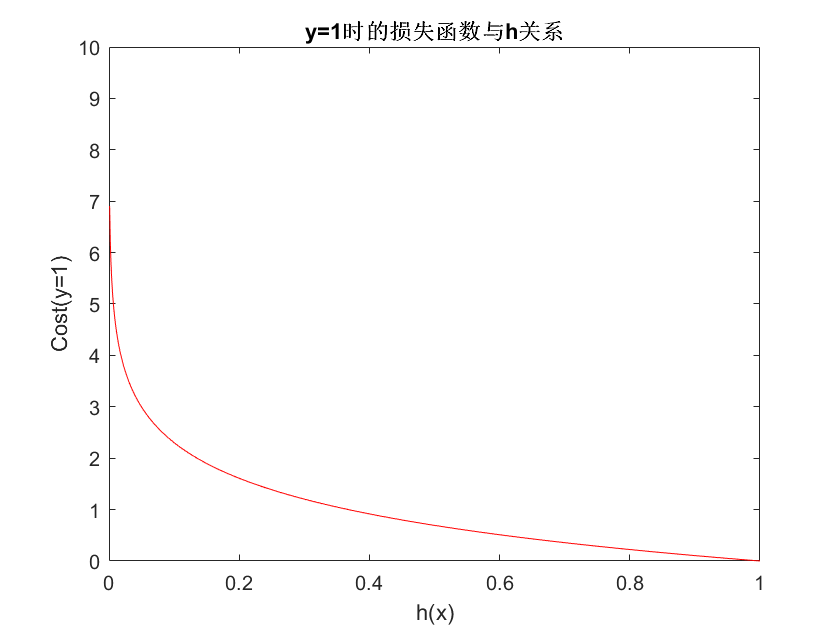
\includegraphics[width=0.6\textwidth]{SigmoidCost1.png} % requires the graphicx package
   \caption{Cost函数与h的关系(y=1)}
   \label{fig:sigmoidcost1}
\end{figure}

\begin{figure}[htbp]
   \centering
   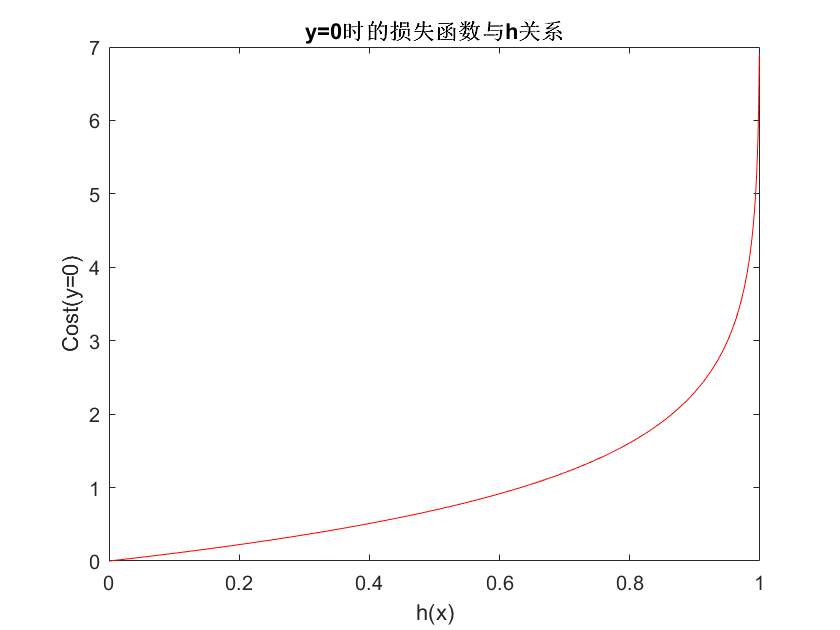
\includegraphics[width=0.6\textwidth]{SigmoidCost0.png} % requires the graphicx package
   \caption{Cost函数与h的关系(y=0)}
   \label{fig:sigmoidcost0}
\end{figure}

可见当$y=1$时,函数一边趋向于0,一边趋向于无穷大;反之亦然。那么,根据其表达式,损失函数可以进一步化简合并为:
\begin{equation}
E(\mathbf{w}) = -\dfrac{1}{m} \sum^m_{i=1} [y^{(i)}log(h(x^{(i)},\mathbf{w})) + (1 - y^{(i)})log(1 - h(x^{(i)},\mathbf{w})) ]
\end{equation}

相应地,我们可以求其一阶导数的表达式如下:(具体推导略)

\begin{equation}
\dfrac{\partial}{\partial w_j} E(\mathbf{w}) = \sum^m_{i=1} (h(x^{(i)}) - y^{(i)})x^{(i)}_j
\end{equation}

这样我们就可以利用之前总结的梯度下降法或者相应的方法进行权重值$\mathbf{w}$的训练。

在进行预测时,如果$y_i>0$,我们则预测相应自变量x对应分类`1';反之预测其对应分类`0'。 

对于多类别的分类问题,我们可以简单地将其划归为多个二分类问题进行处理(称为one-VS-all方法):

比如,当标签$y\in {0,1,2,...,n}$时,我们可以建立一组假设:
$$
\begin{aligned}
h^{(0)}(x,\mathbf{w}) & = & P(y=0|x;\theta)\\
h^{(1)}(x,\mathbf{w}) & = & P(y=1|x;\theta)\\
...\\
h^{(n)}(x,\mathbf{w}) & = & P(y=n|x;\theta)\\
\end{aligned}
$$
最终的预测值$pred = arg\, max_i (h^{(i)}(x))$。

分类问题有很多种解决方法: Softmax函数方法,k-means分类法,支持向量机(Support Vector Machine)方法,决策树方法\cite{standford_machine_learning_cs229};其体现的精神实质是大致相同的,在此就不一一赘述了。

\subsubsection{神经网络}
以上我们讨论了回归、分类问题最具代表性的处理方法。然而,我们可以发现以上模型在面对较高维度输入的时候面临着一些困难: 我们以回归问题为例,当自变量X的具有100维度时,我们考虑先验的$y(x_1, x_2, ..., x_100)$包含项的数目。 我们假设每一个幂项的最高指数为10,没有任何先验的非线性项,那么表达式
\begin{equation}
\begin{aligned}
y(x,\mathbf{w}) = & w_0 + w_{10} x_1 + w_{20} x_1^2 + ... + w_{M0} x_1^M + w_{01} x_2 + w_{02} x_2^2 + ... \\
& + w_{0N} x_2^N + w_{11} x_1 x_2 + ...+ w_{ij} x_1î x_2^j + ... + w_{k} f(x_1, x_2)
\end{aligned}
\end{equation}
中至少有:$100^{10}$项。 

我们发现,随着问题输入规模的扩大,学习的复杂度(体现在权重值$\mathbf{w}$的维度上)呈指数增加的态势。 传统的统计优化方法不再直接适用。

这时,计算机科学家转向了生物学寻求帮助。 生物学上来讲,人类大脑接收信息的维度都极其之高:举例来说,视网膜的分辨率可以达到每英寸300$\sim$400个像素点,然而大脑可以低功耗、低处理成本地进行视觉处理。 大脑里面神经的处理方法很值得我们进行借鉴学习。

生物学研究表明,大脑内部的神经连结成一个复杂的网络;对于大多数神经元,存在多条突触结构与其他神经元相连接,当某一条突触结构上(树突)产生一个高位电信号\textbf{高过一定阈值}时,神经元被激活,通过轴突向其他神经元传播电信号。突触的结构会因为刺激信号的强弱而不断受到训练,神经元之间的连接程度会有所改变。

基于以上规律,我们将讨论一种重要的模型结构——\textbf{神经网络},这是后面深度学习处理的基础。 我们先考虑一个最简单的二层神经网络。
\begin{figure}[htbp]
   \centering
   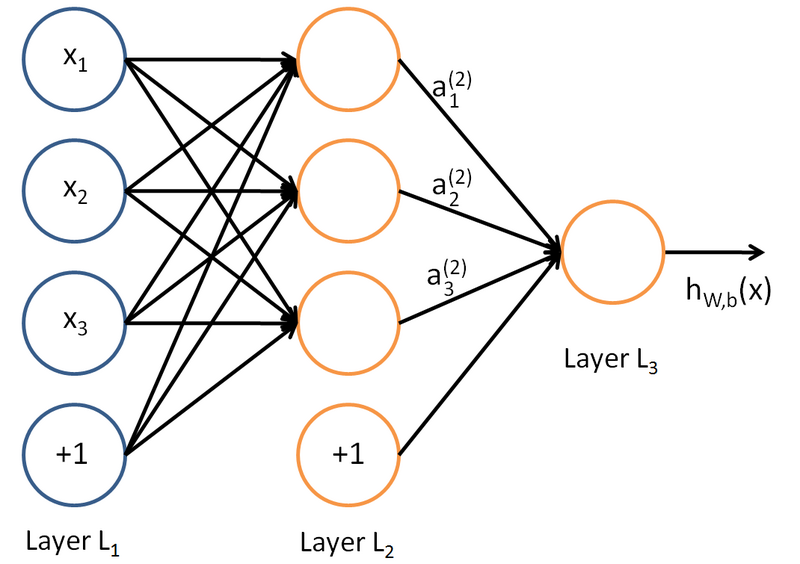
\includegraphics[width=0.7\textwidth]{NeuralNetwork.png} % requires the graphicx package
   \caption{二层神经网络结构示意}
   \label{fig:neuralnetwork}
\end{figure}


如图\ref{fig:neuralnetwork},$a^{(1)}$为输入层,其接收输入信号$x = {x_1, x_2, ... x_{N-1}}$,以及附加一个偏置的常数神经元$a^{(1)}_0$。

$a^{(2)}$为中间层,其中每一个神经元(除了偏置神经元)都与输入层的神经元建立了连接关系,我们假设输入层第$i$个神经元与中间层第$j$个神经元之间的联系权重为$w^{(1)}_{j,i}$。权重值反映两个神经元之间的连接情况:$w^{(1)}_{j,i}=0$反映出两个神经元之间没有连接,$w^{(1)}_{j,i}=1$(归一化以后)反映出两个神经元有很强的正连接关系。其归一化以后的取值范围应当为$[-1,1]$。

我们为了模拟\uline{过阈值激活}的过程,通过sigmoid函数建立起中间层神经元信号强度$a^{(2)}$与输入层信号输入的关系:
\begin{equation}
z^{(2)}_j = \sum^{N_1}_{i = 0} w^{(1)}_{j,i} a^{(1)}_i,\;\; a^{(2)}_j = g(z^{(2)}_j )
\end{equation}
当输入层神经信号的加和值$a^{(2)}_j$超过了阈值“0”的时候,神经元表现为被激活的状态,$z^{(2)}_j$值为1。反之则未激活。

$a^{(3)}$为输出层,其与中间层的连接关系类似与前两层的连接关系:
\begin{equation}
z^{(3)}_j = \sum^{N_2}_{i = 0} w^{(2)}_{j,i} a^{(2)}_i,\;\; a^{(3)}_j = g(z^{(3)}_j )
\end{equation}

神经网络可以应用于回归问题或者是分类问题。

对于一个输入变量x为100维,输出变量y为1维的回归问题,我们可以设置输入层神经元个数$N_1$为100(不包括偏置神经元),用于对应输入$x_1,...,x_100$,设置输出层神经元个数$N_3$为1,中间层设置神经元个数可以自己进行优化,一般设置为$\sqrt{N_1 N_3}$,即设置为10个神经元。 输出层的输出位置我们不再加入Sigmoid函数进行处理,而是直接输出中间层的加和结果:$y = \sum^{N_2}_{i=0} w^{(2)}_{i} a^{(2)}_i$。

此时我们\uline{不再设置各种高阶幂项、交叉项与非线性项的输入},这正是神经网络方法的优势:\uline{sigmoid函数能够较好地处理非线性问题}。通过这样的方法,即使没有高维度的输入变量的假设形式(各种高阶幂项、非线性项),也能够得到较好的结果。在此就不深入探讨原因了,详见\cite{standford_machine_learning_cs229}中的有关讨论。

对于一个输入变量x为400维,标签y为10维的回归问题,应该有:$N_1 = 400, N_2 = 30, N_3 = 10$,此时我们在输出端也加上Sigmoid函数,通过取\uline{输出值里面最大的值}的方法进行预测。

以上我们介绍了利用神经网络的基本结构,以及通过向前传播进行回归、分类预测的方法;然而,如何训练权重值呢? 限于篇幅原因,我们不详细展开讨论,只将结果列出:

首先,神经网络的整体损失函数具体形式为:
\begin{equation}
\begin{aligned}
E(\mathbf{w}) & = [\dfrac{1}{m} \sum^m_{i=1} E(w;x^{(i)},y^{(i)})] + \dfrac{\lambda}{2} \sum^{L-1}_{l=1} \sum^{N_l}_{i=1} \sum^{N_{l+1}}_{j=1} (w^{(l)}_{j,i})^2 \\
& = [\dfrac{1}{m} \sum^m_{i=1}(\dfrac{1}{2}||h(x^{(i)},\mathbf{w})-y^{(i)}||^2)] + \dfrac{\lambda}{2} \sum^{L-1}_{l=1} \sum^{N_l}_{i=1} \sum^{N_{l+1}}_{j=1} (w^{(l)}_{j,i})^2
\end{aligned}
\end{equation}

其中l表示层序数,L为总层数(此处L=3)。$E(w;x^{(i)},y^{(i)})$

为了展开优化,我们需要求出整体损失函数的导数。损失函数对于不同层的导数值求解难易不同,最后一层的w值导数可以直接求得,而E对于前面的每一层w的导数值需要知道后面层数导数值的结果。

因此,我们采用一种“反向传播”的方法求解$E$对于每一层的$w^{(l)}_{j,i}$的导数值\cite{deep_learning_ufldl},具体步骤如下:
\begin{enumerate}
\label{enu: backprop}
\item 由当前的$w^{(l)}_{j,i}$值和输入的$x_i$值进行神经网络的前向传导,得到每一层的激活值$a^{(l)}_j$;
\item 根据输出层的激活值(即预测值$h(x)$)和标签值y计算最后一层的残差:
\begin{equation}
\delta^{(L)}_i = \dfrac{\partial}{\partial z^{(i)}_i} \dfrac{1}{2} ||y - h(x,\mathbf{w})||^2 = -(y_i - a^{(L)}_i) \cdot g^\prime (z^{(L)}_i)
\end{equation}
其中g(z)为Sigmoid函数。那么我们已知其导数值:$g^\prime(z^{(l)}_i) = g(z^{(l)}_i)(1-g(z^{(l)}_i)) = a^{(l)}_i(1-a^{(l)}_i)$。
\item 由最后一层逐层反向计算$l = L-1, L-2, ...2$各层的残差值:
\begin{equation}
\delta^(l) = (\sum^{N_{l+1}}_{j=1}(w^{(l)}\delta^{(l+1)})) \cdot g^\prime (z^{(l)}_i)
\end{equation}
\item 由每层的残差计算相应的导数值:
\begin{equation}
\begin{aligned}
\dfrac{\partial}{\partial w^{(l)}_{j,i}} E(w;x,y) & = & a^{(l)}_i \delta^{(l+1)}_j \\
\dfrac{\partial}{\partial w^{(l)}_{j,0}} E(w;x,y) & = & \delta^{(l+1)}_j
\end{aligned}
\end{equation}
\end{enumerate}

至此,我们已经计算出某一个训练样本的损失函数对于所有$w^{(l)}_{j,i}$权重的偏导数值。

我们将整个神经网络的一个传导、训练的迭代过程总结如下:
\begin{enumerate}
\item 对于所有l,令$\Delta w^{(l)} := 0$,此矩阵用于累加所有训练样本的导数值。(见下过程)
\item 对于所有样本($t = 1\sim m$):
    \begin{enumerate}
    \item 执行上面列表\ref{enu: backprop}里的反向传播过程,计算得到:$\nabla_{w^{(l)}}E(w;x,y)$
    \item 计算
    $$\Delta w^{(l)}:= \Delta w^{(l)} + \nabla_{w^{(l)}}E(w;x,y)$$
    \end{enumerate}
\item 进行权重值的更新过程:
\begin{equation}
\begin{aligned}
w^{(l)} = w^{(l)} - \alpha [(\dfrac{1}{m}\Delta w^{(l)}) + \lambda w^{(l)}] 
\end{aligned}
\end{equation}
\end{enumerate}

通过以上过程就可以进行神经网络的训练过程。

\subsubsection{Bayes公式与机器学习}
作为监督学习的最后一节,我们来讨论一些机器学习的数学基础。大多数机器学习的理论可以通过概率统计的知识,尤其是Bayes理论来进行合理地解释。

Bayes公式又称为逆概率公式。我们假设$D$为观测到的数据,$h$为我们的假设:当h离散时问题为分类问题;当h连续时问题为回归问题。 我们以分类问题为例。$h\in{h_0,h_1,..h_n}$表示最终的分类的可能性。那么Bayes公式表示为:
\begin{equation}
P(h|D) = \dfrac{P(D|h)\,P(h)}{P(D)}
\end{equation}

其中$P(h|D)$称为观测到数据D之后的\textbf{后验概率},$\{P(h_1|D),P(h_2|D),...,P(h_n|D)\}$一组后验概率(其和应当为1)称为数据D观测后的\textbf{信度状态};
$P(D|h)$反映\uline{在假设h下观测到数据D的可能性},称为\textbf{似然函数};
$P(h)$反映\uline{在观测数据D之前对分类h概率的假设},称为\textbf{先验概率};
$P(D)$反映出观测到数据D的概率。

举一个通俗的例子,我们假设大学里面有N名学生,其中男生标记为“Male”,女生标记为“Female”,其他性别为“?”;穿裤子的学生标记为“Pant”,穿裙子的学生标记为“Dress”。

假设我们在路上碰到一个穿裤子的学生,那么我们认为这个学生为男生的概率为

$$P(Male|Pant) = \dfrac{P(Pant|Male)P(Male)}{P(Pant)}$$。其中似然概率反映“如果他是男生,那么他穿裤子的概率”,先验概率反映“走在街上可能碰到男生的概率”。

有时候我们并不关心概率的绝对值,而是关心相对比例,即“碰见一个穿裤子的人,推断其性别的分布情况”,这时分母P(Pant):“走在路上碰到穿裤子的人的概率”不再重要,公式可以简化为:

$$P(Male|Pant) \propto P(Pant|Male)P(Male)$$

先验概率反映出我们对问题观测前的假设。比如,我们大概会认为其他性别的人$P(?)$为0;如果在中国科技大学,男女比大概是4:1,那么P(Male)=0.8,P(Female)=0.2,P(?)=0。 

似然概率反映我们对数据组{D}结构的研究。比如,假设我们通过大量校内抽查,已知男生都穿裤子,女生穿裤子和裙子各占一半,则P(Pant|Male)=1,P(Pant|Female)=0.5。

那么最终$P(Male|Pant):P(Female|Pant):P(?|Pant) = 8:1:0$,我们此处并没有使用到P(Pant)的数据。

将上述模型普适化,则有:

\textbf{后验概率 $\propto$ 似然概率 $\times$ 先验概率}

我们假设对数据没有任何先验认识,比如面对需要拟合的10个点(如图\ref{fig:fitting}),不知道应该用什么曲线进行拟合;

我们的策略是输出极大似然假设——假设的预测值和训练的标签误差平方和最小化。

在\uline{假设数据点围绕真实值高斯分布,并且相互独立时}(正如公式\ref{eqn:random}所描述)可以证明\cite{standford_machine_learning_cs229}:

\uline{能够让数据点在曲线上概率最高的曲线(极大似然曲线)就是使数据点标签值和曲线预测值误差平方最小的曲线}。

极大似然概率和高斯独立同分布为我们前几节损失函数平方和的形式进行了极佳的说明。

先验概率也有很重要的作用。我们曾经提到过\uline{“过拟合”}的现象。10个点的曲线,如果我们用10阶的多项式进行拟合,可以使似然概率达到最大;然而曲线往往不符合现实情况。一种解释角度便是,我们对于曲线具有“阶数较低,平滑”的先验假设,使得10阶拟合曲线的后验概率反而不如3阶曲线的后验概率。

从以上论述可以看出,对于大多数神经网络、曲线拟合的方法,其选择损失函数的形式基本上基于\uline{平衡似然概率与先验概率两方面}。

本论文关注的深度学习算法--深度时空关系推断网络(DeSTIN)也将在第三章详细地用Bayes概率的方法进行理论分析。

\subsection{非监督学习}
以上我们介绍了几种典型的监督学习方法以及相应的Bayes公式原理。监督学习的任务较为明确:\uline{通过训练使得预测值能够较好地符合用于训练的标签值(同时防止“过拟合”)}。然而存在另外的非监督学习机制,其并无训练标签y,但其想通过一些方法获得输入数据$\{x\}$的内部结构,比如说:寻找聚类(Cluster)、主元分析等等。

接下来笔者将介绍一些最常见的非监督学习及其思想。

\subsubsection{k-means聚类方法}

对于非监督学习,其学习任务不再是“使得预测值很好地符合标签值”,一种常见的非监督学习任务便是:寻找输入数据的\uline{聚类情况}。在此,我们对聚类下一个数学定义:

当定义在数据空间$S$的输入的数据点的集合为$\{x\}$时,我们想寻找一个对数据空间的分割$D$,其分为k个部分,这个分割满足以下的性质:
\begin{equation}
D = arg\;min \sum^k_{i=1} \sum_{x_j\in D_i} ||x_j - \mu_i||^2
\end{equation}
其中每一个聚类的具有一个中心位置$\mu_i$;$D = {D_i}$是数据空间$S$被分割后产生的子空间。

我们将上式$\sum^k_{i=1} \sum_{x_j\in D_i} ||x_j - \mu_i||^2$作为损失函数,将聚类的中心位置$\mu_i$作为优化变量,通过极大似然分析,就可以得到一种简单易行的聚类方法,称为\uline{k-means聚类方法},其具体过程如下:
\begin{enumerate}
\item 在数据空间S中,随机生成k个聚类中心位点,其代表k个聚类;
\item 将数据集$\{x_j\}$中的点分配到\uline{最近的聚类中心}代表的聚类中去【分类规则】;
\item 计算每一个聚类集合内部数据点的平均值(质心)位置,并将其作为新的k个聚类的中心【更新规则】;
\item 重复前两步,直至聚类结果不再变化。
\end{enumerate}

典型的k-means过程如图\ref{fig:kmeans}。

\begin{figure}[htbp]
   \centering
   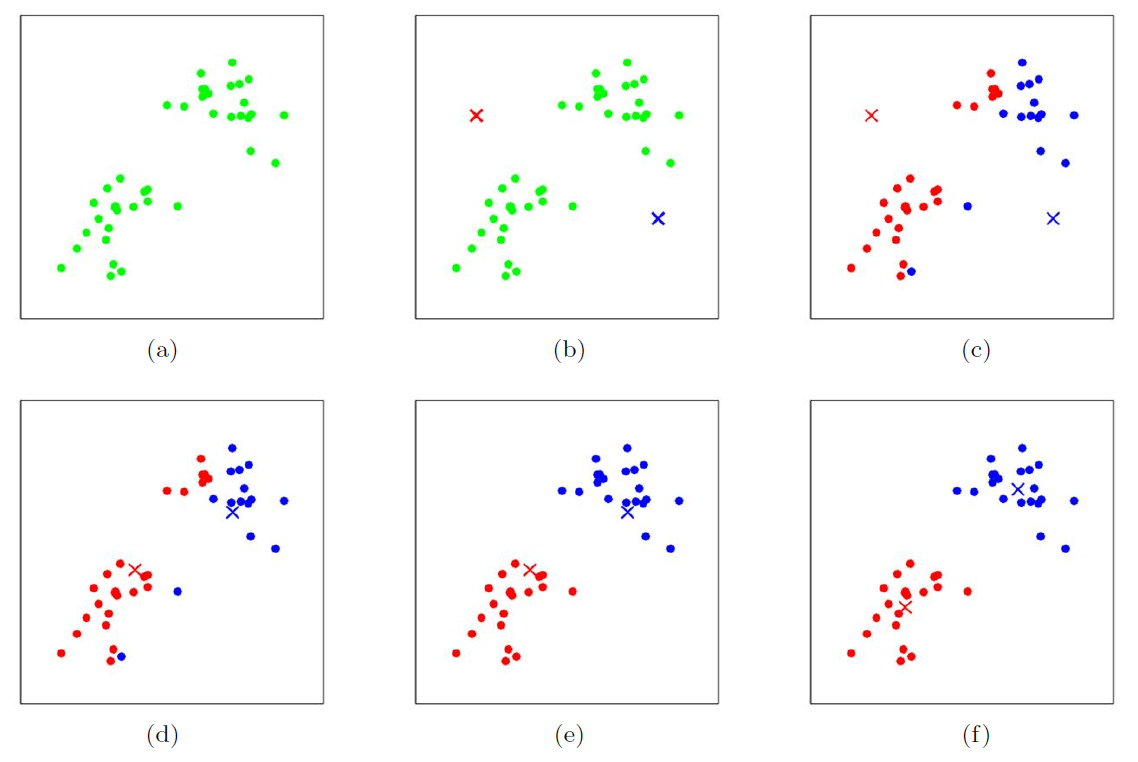
\includegraphics[width=0.7\textwidth]{kMeansClustering.png} % requires the graphicx package
   \caption{k-means聚类分析过程:“×”形代表聚类中心。}
   \label{fig:kmeans}
\end{figure}

可以发现,k-means算法的计算量相当大:每一次更新过程都要重新计算每一个样本点到聚类中心的距离。如果数据集容量较大,或者是数据集本身在持续更新(实时系统),采用上述的k-means算法可能不太合适。我们可以更改更新规则,使其变为一个在线的k-means算法(Online k-means Clustering Algorithm):

\begin{enumerate}
\item 在数据空间S中,随机生成k个聚类中心位点,其代表k个聚类;
\item 读入一个观测数据,称为$in_j$,寻找距离其最近的聚类中心,将其分配到该“获胜”的聚类中:
\begin{equation}
i \leftarrow arg\;min_i ||in_j - \mu_i||
\end{equation}
\item 通过输入的观测数据$in_j$,来更新“获胜”的聚类中心位置$mu_i$。
\begin{equation}
\mu_i \leftarrow \mu_i + \eta(in_j - \mu_i)
\end{equation}
其中$\eta$是人为调整的一个学习速率。
\item 重复之前两步,直到某一个满足终止规则为止。
\end{enumerate}

这种方法又称为“Winner-Take-All”聚类方法,因为每一次只有一个最近的聚类被更新。学习速率$\eta$的规定也将相当重要。如果$\eta$一直保持一个常数,那么这种聚类算法将不会收敛(这对于某些实时更新的系统是必要的);如果$\eta$按照某个规律衰减,那么后输入的数据对于聚类产生的影响将逐渐变小,可能导致聚类规则不准确。

另一种聚类方法的扩展称为“结构性聚类”(hierachical clustering)。这种方法基于“聚类具有子聚类”的思想。 在一种具体的结构性聚类方法(Agglomerative Hierarchical Clustering)里面,\cite{Duda2001Pattern}
每一个数据点$x_i$一开始都代表一种聚类$D_i$。算法不断地结合相隔最近的两个聚类,直到聚类总数减少到k为止。

我们后面讨论的深度空时学习网络采用了“在线聚类方法”作为神经节点的更新规则;同时也借鉴了“结构性聚类”方法的“聚类具有结构性”的思想。

\subsubsection{Gaussian混合聚类模型}
我们分析k-means聚类的统计学实质可以知道:

上述的k-means方法的损失函数$\sum^k_{i=1} \sum_{x_j\in D_i} ||x_j - \mu_i||^2$是基于独立的Gaussian聚类的:就是说,我们是假设存在数据空间$S$中存在k个独立的Gaussian分布$\{\mu_i, \Sigma_i\}$,假设每个数据$x_j$\textbf{只属于其中的一个Gaussian聚类},通过极大似然的方法用数据集$\{x_j\}$反推独立的Gaussian分布$\{\mu_i, \Sigma_i\}$的参数的过程。

然而对于不同聚类交叠较为严重的问题,k-means的处理方法并不是非常合适。
\begin{figure}[htbp]
   \centering
   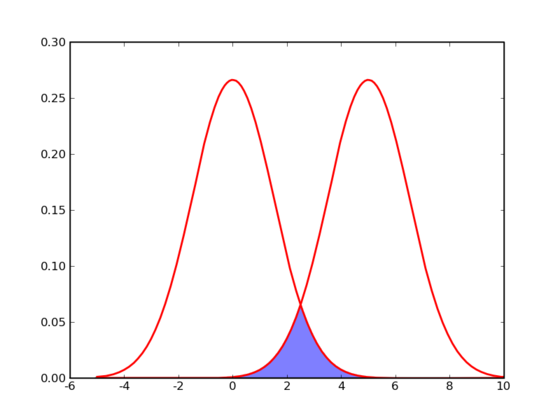
\includegraphics[width=0.5\textwidth]{kMeansProblem.png} % requires the graphicx package
   \caption{k-means聚类之难:交叠处(x=2.5)到底属于哪一个聚类?}
   \label{fig:kmeansproblem}
\end{figure}

如图\ref{fig:kmeansproblem},当我们分析x=2.5处的数据点属于哪一个聚类时,很难一刀切地通过微小的离聚类中心距离$||x_j - \mu_i||$的差距来断定聚类属性。

这时候我们产生了另一种模型,称为Gaussian混合聚类模型,其模型假设如下:

数据空间$S$中存在k个Gaussian分布的聚类$\{\mu_i, \Sigma_i\}_{i = 1\sim k}$;
空间中每一个点$x$存在一定概率属于其中每一个聚类,概率分别为$\{w_i\}$,其构成一个概率向量$\mathbf{w}$; 这样的概率向量在数据空间$S$中为一个连续的函数$\mathbf{w}(x)$。

在给定聚类属性$\{\mu_i, \Sigma_i\}_{i = 1\sim k}$和聚类概率分布$\mathbf{w}(x)$的情况下在x处观测到数据的似然概率为:

\begin{equation}
p(x|\{\mu_i, \Sigma_i, w_i \}) = \sum^k_{i=1} w_i g(x|\mu_i, \Sigma_i)
\end{equation}

其中$g(x|\mu_i, \Sigma_i)$为x单独在第i个Gaussian分布中被观测到的概率。

我们将Gaussian聚类属性参数和概率分布合并表示,称为模型假设:
$$\lambda_i(x) = \{\mu_i, \Sigma_i, w_i(x)\}, \; \lambda = {\lambda_i}$$

那么我们可以反推出在模型假设$\lambda$下,观测到数据集$\{x_j\}$的概率:

\begin{equation}
p(\{x_j\}|\lambda) = \prod^m_{j=1} p(x_j|\lambda)
\end{equation}

至此,我们可以通过极大似然概率来反解$\lambda = \{\mathbf{w}, \mathbf{\mu}, \Sigma \}$

我们假设样本点彼此相互独立,那么数据\uline{不存在协方差},高斯分布$\Sigma_i$项中不含非对角项。

为了让极大似然概率达到最大,我们可以采用一种期望值最大化算法(Expectation Maximization Algorithm),通过重复地迭代以下过程,我们可以获得需要的参数$\lambda$:
\begin{equation}
\left\{
\begin{aligned}
w_i & = & \dfrac{1}{m} \sum^m_{j=1} P(i|x_j, \lambda)\\
\mu_i & = & \dfrac{\sum^m_{j=1} [P(i|x_j, \lambda)]\, x_j}{\sum^m_{j=1} P(i|x_j, \lambda)} \\
\sigma^2_i & = & \dfrac{\sum^m_{j=1} [P(i|x_j, \lambda)]\, x_j^2}{\sum^m_{j=1} P(i|x_j, \lambda)} - \mu^2_i
\end{aligned}
\right.
\end{equation}

\begin{equation}
P(i|x_j, \lambda) = \dfrac{w_i g(x_j|\mu_i, \Sigma_i)}{\sum^k_t w_i g(x_j|\mu_i, \Sigma_i)} 
\end{equation}

我们的算法(DeSTIN)同样借鉴了混合聚类的思想:每一个数据点并不是确定性地属于一个聚类,其具有属于每一聚类的概率。

\subsubsection{自编码神经网络}

以上我们讨论了两种典型的聚类方法。接下来我们讨论另一种常见的非监督学习问题:主元分析(Principal Component Analysis)。 

主元分析的目标是:通过原始数据变量的线性组合,构造一组新的变量;这组新变量之间互相不相关,并且尽可能地做到了信号压缩:用尽可能少的变量表示所有的信息。

\begin{figure}[htbp]
   \centering
   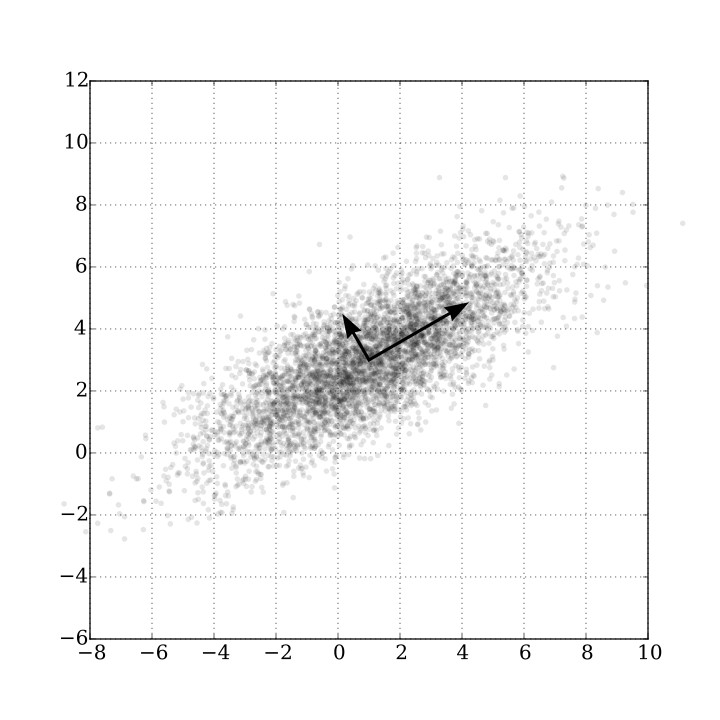
\includegraphics[width=0.5\textwidth]{PCAGaussian.png} % requires the graphicx package
   \caption{主元分析对于Gaussian分布数据的影响}
   \label{fig:pca}
\end{figure}

如图\ref{fig:pca},在原坐标下,一组二变量Gaussian分布的数据有较强的坐标相关性;通过主元分析,我们找到了一组新的坐标,在该坐标下,Gaussian分布被对角化了,并且信息集中在了一根坐标轴上。

常用的进行主元分析的方法是\uline{奇异值分解}。我们假设数据集为:$\hat{X} = [x^{(1)}; x^{(2)};...; x^{(m)}]$,对其进行奇异值分解后的结果是:

$$\hat{X} = USV^T$$

设$T_D = US$,我们假设将原坐标$\{\hat{a}\}$映射到主元的新坐标$\{\hat{b}\}$的变换矩阵为$T_L$,那么$T_L$即为$T_D$的前L列。

有趣并且有启发性的是,我们可以通过一种简单的神经网络结构获得相似的结果,其称为自编码神经网络(Auto-encoders)。

为了解决非监督学习没有训练标签的问题,我们不妨\uline{让数据本身作为标签}。

\begin{figure}[htbp]
   \centering
   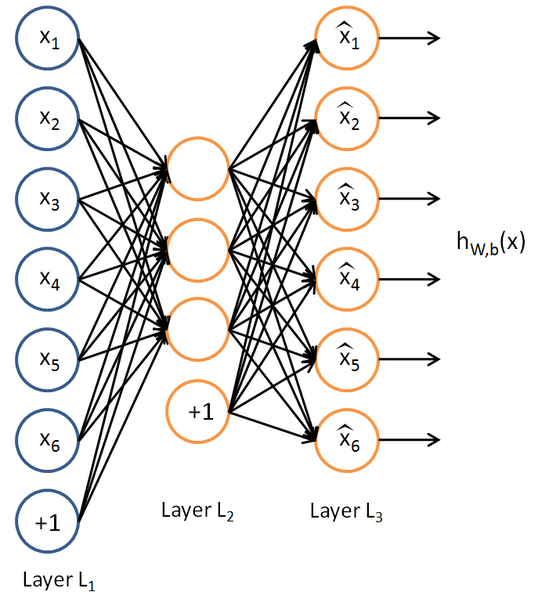
\includegraphics[width=0.5\textwidth]{Autoencoder.png} % requires the graphicx package
   \caption{自编码神经网络结构示意}
   \label{fig:pca}
\end{figure}

自编码神经网络尝试学习$h_w(x)\approx x$的函数,这件事情看上去不太有意义,但是当我们将中间层神经元数目减少时,我们可以驱使神经网络去学习数据的\textbf{压缩表示}。 

自编码神经网络的学习训练方法同上一节监督学习中的神经网络一致,而其隐藏层的神经单元往往隐含了主元分析类似的有效信息结果。

\section{深度学习}
以上我们对机器学习代表性的思想和方法进行了一个回顾, 接下来我们对机器学习的一个分支--深度学习做一个基本的介绍。

%为什么需要深度学习呢?我们已经在第一章\ref{chapter_introduction}进行过一些说明。

深度学习的背景是人工智能的发展。我们希望通过机器学习的方法构建起一个\uline{智能系统},而智能系统的基础就是\uline{其能够利用有限的资源有效地解决大量特征、高维度数据下的机器学习问题}。而传统方法下,为了处理过于复杂的问题,我们总是对数据做很多预处理,通过先验知识将问题化归到小特征空间上去,这样的方法过于困难,并且缺乏通用性。\cite{Duda2001Pattern}

深度学习的目的就在于突破学习算法的“维度困境”\cite{bellman1957dynamic},通过多层网络结构来实现高维度信息的处理。

从结构上来说,深度学习结构定义为一个包含多层非线性变换的模型。\cite{bengio2009learning}除数据的输入层外,每一层的输入信号都由前面一层的输出产生;通过一些监督、非监督学习的学习方法,输出数据给下一层结构。

从功能上来说,深度学习尝试从未经人为处理的现实的高维度数据中直接进行特征学习。比如,在没有给机器任何的先验信息的前提下,给出大量的真实照片,让机器自己去提取照片里面的物体、进行边缘检测等等。

深度学习的核心部分在于\uline{如何从海量的数据里面提取有效特征},即特征提取。每一层提取到的特征随着层数变深逐渐全局化。最终我们可以利用不同层的提取的特征进行后期的监督学习(回归、分类)或者非监督学习(聚类、主元分析)。

深度学习起源于神经网络的研究。普通的神经网络只包含了一层隐藏层,当我们将隐藏层拓展为多层时,就成为了“深度神经网络(Deep Neural Network)”。研究发现\cite{bengio2009learning},深度神经网络具有较普通神经网络更加好的非线性特征提取能力。然而,深度神经网络的问题在于:
\begin{enumerate}
\item 过拟合现象: 由于神经网络的参数过多,数据量不够导致过拟合容易发生;
\item 局部极值问题: 使用监督学习方法训练深度网络时,求解的损失函数往往是高度非凸的优化问题,存在各种局部极小值点,使得梯度下降类的方法效果不好;
\item 梯度弥散问题: 梯度下降法的另一个问题是,随着网络深度增加,反向传播的梯度值会急剧减小,以至于最初的几层神经网络无法进行有效的学习;
\item 训练过程非常耗时,消耗计算资源;算法效率低。
\end{enumerate}

为了解决过拟合的问题,陆续有很多正则化的方法提出;一个更加有效的方法是,“随机剔除(dropout)”方法\cite{JMLR:v15:srivastava14a},即在训练的过程中随机地关闭掉一些隐藏层的神经元,以防止整个系统产生一些特定的对于神经元的依赖关系。另外一个解决过拟合的方面是,我们需要获取足够多的样本:足量的数据能够保证过拟合现象不会发生。

而为了解决局部极值、梯度弥散两个问题,学界诞生了一种“逐层贪婪训练”的方法:每一次只训练一层网络,当这一层网络训练结束以后,固定之前训练的所有k-1层网络(不再训练),增加第k层在网络的最后进行学习(通常用自编码器进行无监督学习);各层单独训练后的权重当做整体训练的初始值,然后对整个网络进行监督训练,获得“微调”效果。具体过程参见\cite{deep_learning_ufldl}。


最后,为了更有效地提取特征,提高算法效率,两种重要的基于以上思路的改进产生了的新的深度学习算法:\uline{卷积神经网络}\cite{hinton2006fast}与\uline{深度信度网络}\cite{lee2009convolutional}。这两种算法的产生标志着深度学习方法的成熟化。本节接下来简要介绍这两种深度学习算法。

\subsection{卷积神经网络}
卷积神经网络(Convolutional Neural Network,CNN)在处理2D图像的问题上取得了成功。我们主要围绕其在图像处理上基于深度神经网络进行的改进进行说明。

\subsubsection{部分联通网络的必要性}
我们已经知道传统“深度神经网络”(DNN)面临的最终困难:“全连接”的神经网络非常消耗计算资源和时间:我们以一层隐藏层的神经网络为例:

当输入数据维度为n,标签维度为k时,第一层神经元个数为n个,第二层假设为$\sqrt{nk}$个,第三层为k个;那么其需要的总权重参数数目为:

$N(\mathbf{w}) = (n+1)\cdot\sqrt{nk} + (\sqrt{nk}+1)\cdot k \propto n\sqrt{n}$

假如我们的输入数据为手机屏幕图片,其维度量级大致为100*100像素点;假设你要学习图像的100个特征,那么我们需要的参数$N(\mathbf{w})$量级大概是:$100*100*\sqrt{100*100*100} = 10^7$。

对于高维度数据,全连接(指每一层所有神经元与其相邻一层所有神经元相连接)神经网络不符合现实。我们应当采用\textbf{部分联通网络}的结构:\uline{每一个神经网络仅连接输入单元的一部分},对于图片来说,可能是相邻区域。

\begin{figure}[htbp]
   \centering
   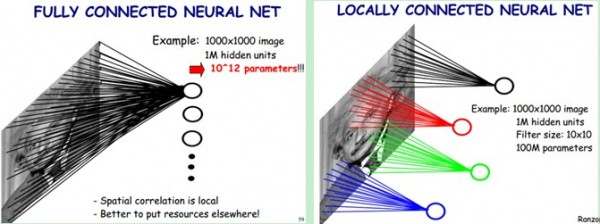
\includegraphics[width=0.7\textwidth]{LocallyConnectedNetwork.jpg} % requires the graphicx package
   \caption{部分连接网络示意}
   \label{fig:localnetwork}
\end{figure}

网络部分联通(locally connectivity)的思想,也是受启发于生物学里面的视觉系统:视觉皮层的特定神经元只由相应某些特定视网膜区域才能刺激。

仍然是100*100的像素点输入层,假如第二层的神经元只和附近的10*10个像素点相连,那么权重值的数目降到了原来的百分之一。假定原来第二层有100个神经元,原权重值数目为:$100*100*100 = 10^6$;现权重值数目为$10*10*100 = 10^4$。


\subsubsection{图像特征的全局性,参数共享与卷积}
自然图像具有一种特性:同一幅图像的某一块区域的统计特性(比如频谱大小)和其他部分基本相同。 \cite{Hyv2009Natural}这意味着如果我们在某一块小区域学习到了某一个特征,其在图像上其他的位置可能也会有所反映。

这启发我们先在一个小区域进行特征学习,再将该特征对应到整个区域上去。具体来说,我们可以在一个大尺寸图像上随机选取一个小区域(比如$8*8$的小块),通过无监督学习的方法(比如自编码器)进行了特征$\{a\}$的学习;再将该特征$\{a\}$作为一个探测器,应用到图像的任意地方去。

数学上,为了建立起某一个局部区域特征和图像其他位置的作用,我们可以进行\textbf{卷积}操作;笔者简单描述一下二维离散有限域卷积的公式。

设某一$M\times N$的图像对应一个离散$(x,y)$的函数
$f(x,y) \;(x = 1\sim M,y = 1\sim N)$,
其中某一个小区域对应的函数为
$g(x,y) \;(x = 1\sim A, y = 1\sim B)$,那么两个函数卷积的结果是:
$$f*g(x,y) = \sum^{A-1}_{p=0} \sum^{B-1}_{q=0} f(p,q)g(x-p,y-q) \,\; x = 1\sim M-A+1, \,y = 1\sim N-B+1$$

直观的理解,就是将小区域水平、垂直翻转,再与大单元的相应位置单元的值相乘,最后进行求和。如图\ref{fig:conv}所示。我们将对大区域进行卷积的小区域称为\textbf{卷积核}。

\begin{figure}[htbp]
   \centering
   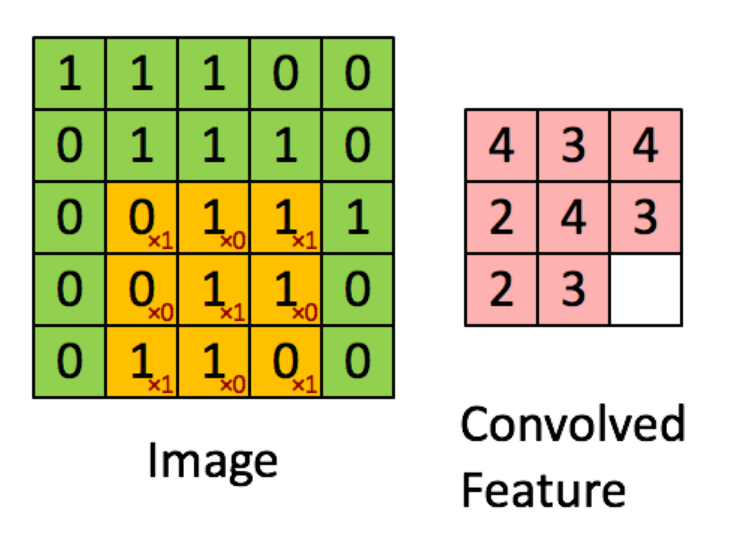
\includegraphics[width=0.6\textwidth]{Convolution.png} % requires the graphicx package
   \caption{二维离散有限卷积示意}
   \label{fig:conv}
\end{figure}

在此我们要\textbf{拓宽卷积的语义}。在以上过程中,卷积核表示图像的一部分区域$g(x,y)$,卷积操作的运算为$\sum g(x-p,y-q)\cdot f(p,q)$,如果我们将卷积核的值看作系数,则有卷积操作变为:
\begin{equation}
Conv(f(x,y))  = \sum_{i,j} w(x-i,y-j)\cdot f(i,j)
\end{equation}

此时卷积已经变为了一种某个区域内(大小为$A\times B$)的元素线性变换再加和的过程。
广义的卷积,就是一个线性变换再求和的过程;此时的\uline{卷积核不再理解为图像的一个区域,而是理解成\textbf{线性变换的系数$w_{i,j}$和尺度}}。

卷积相当于是一种全局的线性算子,其平移并作用于整个图像,进行线性运算并加和,输出特征的卷积结果。

我们将卷积的过程看作一种特殊的神经网络层间过渡过程:假设输入层的数据为$x$,那么卷积层的神经元表示为:
\begin{equation}
\label{eqn:conv}
a^l_{i,j} = g(z^l_{i,j}) = g((w^l \ast x)_{i,j} + b_l)
\end{equation}

其中,$g(z)$为Sigmoid激活函数,$a^l$为卷积层的神经元激活值,$\mathbf{w^l}$作为卷积核充当了之前连接两层神经元的权重值的功能(也将是训练的核心)。$b_l$为常数偏移值,之前都合并在$\mathbf{w^l}$中,在2D模型中为了表示方便,将其提出。

\begin{figure}[htbp]
   \centering
   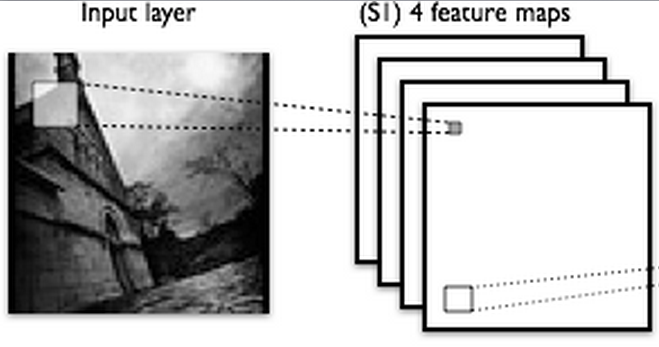
\includegraphics[width=0.6\textwidth]{ConvolutionKernal.png} % requires the graphicx package
   \caption{通过卷积进行输入层到中间层的连接}
   \label{fig:convker}
\end{figure}

%举一个具体的例子描述卷积通道的形成的过程:假设我们有一副$96\times96$的图像,我们选取了一个$8\times8$的区域作为其卷积核:
%\begin{enumerate}
%\item 我们对该$8\times8$的样本区域进行自编码学习,假设其隐含单元数为100;
%\item 学习完成后,我们将抽取的$8\times8$区域同整个图像进行卷积运算
%\end{enumerate}

值得一提的是,我们可以采用自编码器作为卷积核,进行卷积层的相关操作,参见\cite{deep_learning_ufldl}。

对于一幅高维度图像,我们当然不会只提取一个特征。 对于多个特征的情况,我们可以设置多个卷积核,每个卷积核根据\ref{eqn:conv}计算得到一个\uline{卷积通道}(也称为特征图(feature map));最终生成的卷积层成为一个多层的三维结构。可以发现,当前后两层结构都为三维结构时,联系这两层结构的权重值$w^{lk}_{i,j}$将成为四阶张量。

\subsubsection{特征归并:池化}
我们通过卷积核构造出了卷积层,并希望能够进行下一层神经网络的搭建。然而我们面临着计算量的困境:直接卷积得到的卷积层神经元过多。

对于一副$96\times96$的图像,假设我们训练了400个$8\times8$的卷积核,那么每一个卷积核将产生$89^2=7921$维的卷积通道;卷积层的总维度将高达:$89^2*400 = 3168400$。

以下我们介绍对特征进行归并化简的方法:池化(pooling)。池化的操作非常简单:\uline{将每个卷积通道划分为可数的区域,计算每个区域特征的平均值(或最大值)},并将其作为池化后的神经元结果。

池化的合理性在于卷积的平坦性:某一个位置的卷积结果与其相邻位置卷积结果不会相差很多;基于此我们就可以对于图像某个区域进行归并统计。

以上我们介绍了卷积神经网络的主要思想,其训练过程同普通神经网络一样,也采用反向传播算法。由于其提取图像特征的有效性,通常层数比相同效果的深度神经网络要少得多,因而训练将更为迅速。

图\ref{fig:lenet}是一个典型的卷积神经网络(CNN)的结构,其基本构造为:输入的图像先进行卷积核特征提取,再池化;再进行卷积核特征提取,再池化;最后输出到全连接的神经网络中进行监督训练。

\begin{figure}[htbp]
   \centering
   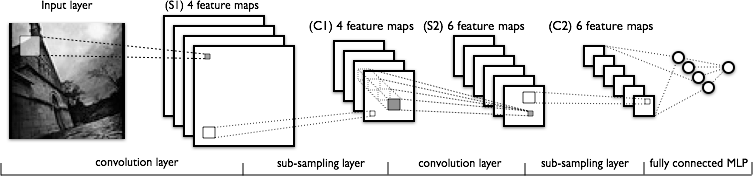
\includegraphics[width=0.8\textwidth]{Lenet.png} % requires the graphicx package
   \caption{典型的卷积神经网络结构(LeNet)}
   \label{fig:lenet}
\end{figure}

\subsection{深度信念网络}
同CNN不同,深度信念网络(Deep Belief Networks, DBNs)是一种直接基于Bayes概率的方法,和原来的神经网络方法有较大的不同。

\subsubsection{受限Boltzmann机模型}
在介绍DBN之前,我们先要介绍构成DBN的基本单元——受限Boltzmann机(Restricted Boltzmann Machine, RBM)。该模型是用于判断数据的属于不同类别的概率的(即分类模型),其优势在于训练较为简单,便于在DBN网络中使用。

\begin{figure}[htbp]
   \centering
   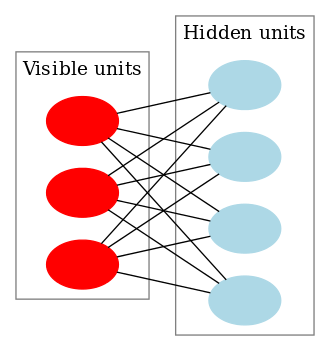
\includegraphics[width=0.4\textwidth]{RestrictedBoltzmannMachine.png} % requires the graphicx package
   \caption{受限Boltzmann机示意}
   \label{fig:rbm}
\end{figure}

如图\ref{fig:rbm},RBM由可见层$\{v_i\}$和隐藏层$\{h_j\}$,可见层的常数偏置单元$\{a_i\}$以及隐藏层的常数偏置单元$\{b_i\}$组成。其中$\{v_i\}$,$\{h_j\}$的值在标准的RBM中只能取0或1。类似于神经网络,我们定义单元之间的连接权重$\mathbf{w} = (w_{i,j})$。

我们定义这个结构的\textbf{能量}为:
\begin{equation}
E(v,h) = - \sum_i a_i v_i - \sum_j b_j h_j - \sum_i\sum_j v_i w_{i,j} h_j
\end{equation}
或者简记为:
$$E(v,h) = -a^T v -b^T h - v^T \mathbf{w} h$$

在这个网络中,$v,h$的联合概率分布可以表示为:
\begin{equation}
P(v,h) = \dfrac{1}{Z} e^{-E(v,h)}
\end{equation}

其中Z为配分函数,即所有$(v,h)$可能取值下$e^{-E(v,h)}$的加和,即归一化系数。

那么容易求得$v$的边缘分布函数为:
\begin{equation}
P(v) = \dfrac{1}{Z} \sum_h e^{-E(v,h)}
\end{equation}

可以发现,RBM是一个双向对称结构;在给定$v$的情况下,$h$的激活情况相互独立;反之亦然。我们可以得到以下条件概率公式:

\begin{equation}
P(v|h) = \prod^m_{i=1} P(v_i|h)\;,\; P(h|v) = \prod^n_{j=1} P(h_j|v)
\end{equation}

每一个单元激活概率由Sigmoid函数g(z)给出:

\begin{equation}
P(v_i=1|h) = g(a_i + \sum^n_{j=1} w_{i,j}h_j )\;,\; P(h_j =1|v) = g(a_i + \sum^m_{i=1} w_{i,j}v_i )
\end{equation}

RBM有着较为简单的训练方法:假设输入训练集为$V = [v^{(1)};v^{(2)};...;v^{(m)}]$ ,RBM的训练目标为使得v的产生概率最大;

\begin{equation}
arg\; max_{\mathbf{w}} \prod_{v\in V} P(v)
\end{equation}

或者等效于:

\begin{equation}
arg\; max_{\mathbf{w}} \sum_{v\in V} log P(v)
\end{equation}

我们仍然可以采用梯度下降法对其进行训练,在此不赘述。

\subsubsection{DBN的结构}

如图\ref{fig:dbn}我们将RBM进行层级堆叠,并且采用“逐层贪心训练”的方法,就可以实现所谓DBN的架构。\cite{hinton2006fast}

\begin{figure}[htbp]
   \centering
   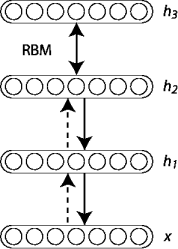
\includegraphics[width=0.4\textwidth]{DeepBeliefNetwork.png} % requires the graphicx package
   \caption{DBN架构示意}
   \label{fig:dbn}
\end{figure}

我们分析DBN能够提取出训练数据层次结构特征的原因:在DBN模型中,观测变量$x$与前$l$层隐藏变量$h^1,h^2,..h^l$的联合概率分布如下:(由RBM模型可推知)

\begin{equation}
P(x,h^1,h^2,...,h^l) = (\prod^{l-2}_{k=0} P(h^k|h^{k+1})) P(h^{l-1},h^l)
\end{equation}

其中$x=h^0$,$P(h^{k-1}|h^k)$反映出第k层RBM的由隐藏层到可见层的条件概率,$P(h^{l-1},h^l)$为第l层RBM的可见层与隐藏层的联合概率。

可见上式构成一个良好的递推结构,那么我们可以从一层RBM训练出发;将底层的隐藏层信息作为上一层的可见层输入,固定底下的层数训练最高的一层;训练完所有层数后再使用监督学习方法进行全局微调,即完成了整个DBN训练过程。

由于DBN大部分内容与本论文无关,此处不展开介绍,详见\cite{lee2009convolutional}。